\label{ch:groups}



%\section{Now it starts}
The identity type is not just any type.  In the previous sections we have seen that the identity type $a=_Aa$ reflects the ``symmetries'' of a term $a$ in a type $A$.  Symmetries have special properties; for instance you can rotate a square by $90^o$, and you can rotate it by $-90^o$, undoing the first rotation.
Symmetries can also be composed, and this composition respects certain rules that holds in all examples.  When coining the concept of ``symmetries'', we should isolate these common rules for all our examples, but also show, conversely, that anything satisfying these rules actually \emph{is} an example.  This is the purpose of the mathematical term ``group''.

As an instance of a property that holds in some examples but not in others, we have seen that sometimes the order in which we use our symmetries matters, and sometimes it does not, see \cref{ch:intro}.  Hence, the concept of a group should not have a rule allowing you to change the order arbitrarily.

In \cref{sec:identity-types} we saw that the identity type was ``reflexive, symmeric and transitive''.

With inspiration of geometric and algebraic origins, it became clear to mathematicians at the end of the 19'th century that the properties of such symmetries could be codified by saying that they form a \emph{group}.

\begin{example}\label{ex:base=base}
  We defined the circle $S^1$ in \cref{def:circle} by declaring that it has a point $\base$ and an element $\Sloop:\base=_{S^1}\base$, and we proved in \cref{lem:S1groupoid} that $\base=_{S^1}\base$ is equivalent to the set $\zet$ (of integers), where $n\in\zet$ corresponds to the $n$-fold composition of $\Sloop$ (which works for both positive and negative $n$).  We can think of this as describing the symmetries of $\base$: we have one ``generator'' $\Sloop$, and this can be applied any number of times, giving a new symmetry for each new number.  Here, composition of loops corresponds to usual addition of integers.  Hence, the circle is a very cheap packaging of the ``{group}'' of integers, the declaration of $\base$ and $\Sloop$ not only gives the set $\zet$ of integers, but at the same time the addition.
\end{example}
\begin{example}
  Recall the finite set $\bn{2} =\bool:\fin_2$ from \cref{def:finiteset}, containing two elements.   
According to \cref{xca:C2}, $\bn{2} =\bn{2} $ has exactly two elements, $\refl{\mathrm 2}$ and $\twist$, and doing $\twist$ twice gives you back $\refl{\bn{2} }$.  
We see that this is exactly all the symmetries you'd expect to have in a two point set: you can let everything be ($\refl{\bn{2} }$) or you could swap the two elements ($\twist$); and if you swap twice everything is let be.  
The type $\fin_2$ (of ``finite sets with two elements'') is our embodyment of these symmetries.  

Observe that (by the definition of $S^1$) there is an interesting function $S^1\to\fin_2$, sending $\base:S^1$ to $\bn{2} :\fin_2$ and $\Sloop$ to $\twist$.
\end{example}


The examples Klein and Lie were interested in were of a type making it admissible to say that a group is the identity type $a=_Aa$ for \emph{some} type $A$ and \emph{some} element $a:A$.
However, in elementary texts it is customary to restrict the notion of a group to the case when $a=_Aa$ is a \emph{set} as in \cref{sec:identity-type-as-abstract}.  This makes some proofs easier, since if are we given two elements $g,h:a=_Aa$, then the identity type $g=h$ is a proposition, \ie $g$ can be equal to $h$ in at most one way.  Hence questions relating to uniqueness will never be a problem.



See \cref{sec:grouphistory} for a brief summary of the early history of groups.
\begin{remark}
  The reader may wonder about the status of the identity type $a=_Aa'$ where $a,a':A$ are different elements.  One problem is of course that if $p,q:(a=_Aa')$ there is no obvious way of composing $p$ and $q$, and another is that $a=_Aa'$ does not have a distinguished element such as $\mathrm{refl{}_a}:a=_Aa$.
Given $f:a=_Aa'$ we can use transport along $f$ to compare $a=_Aa'$ with $a=_Aa$ (much as affine planes can be compared with the standard plane or a finite dimensional real vector space is isomorphic to some Euclidean space), but absent existence and choice of such an $f$ the identity types $a=_Aa'$ and $a=_Aa$ are different animals.
\end{remark}


\begin{remark}
  When considering the identity type $a=_Aa$, only the elements $x:A$ with $x$ equal to $a$ are relevant, and we are free to consider only \emph{connected} $A$, \ie where $x=_Aa$ is always inhabited (c.f.~\cref{def:connected}).  Also, our preference for $a=_Aa$ to be a set indicates that we should consider only the connected types $A$ that are \emph{groupoids}.
\end{remark}


With this established, we let the \emph{type} of groups be defined as follows:

\begin{definition}\label{def:typegroup}\footnote{we must define  $\isset$ and propositional truncation.  Alternatively we must define $\isonetype$ and $\conn$}
  A \emph{group} is a pointed connected groupoid; the \emph{type of groups} is the type 
%$$\typegroup=\sum_{A:\UU}A\times\isonetype(A)\times \conn_0A.$$
$$\typegroup\defequi\sum_{A:\UU}\sum_{a:A}\isset(a=_Aa)\times\prod_{x:A}||x=_Aa||$$
of pointed connected groupoids.
%We refer to an element of $\typegroup$ as a \emph{group}.  
A group $G=(A,a,p,q):\typegroup$ will be referred to simply as $$\aut_A(a).$$  The underlying pointed type $$BG\defequi(A,a)$$ is referred to as the \emph{classifying space of $G$}. 
\end{definition}
\begin{remark}\label{rem:aut}
There is no ambiguity in writing $\aut_A(a)$ instead of $(A,a,p,q)$: being a connected groupoid is asserted by 
$$\isset(a=_Aa)\times\prod_{x:A}||x=_Aa||$$ which is a proposition  (\cref{lem:props-are-props}) and so the witness $(p,q)$  is unique.  In this sense, once you know that the classifying space is a connected groupoid, $BG$ carries all the information about $G$: $$G\oldequiv\aut_{BG_\div}(pt_{BG}).$$
\end{remark}
\end{definition}
   \begin{example}\label{excirclegroup}
   The circle $S^1$, which we defined in \cref{def:circle}, is a connected groupoid (\cref{lem:circleisconnected}, \cref{lem:S1groupoid}) and is pointed at $\base$. The identity type $\base=_{S^1}\base$ is equivalent to to the set of integers $\zet$ and composition corresponds to addition.  This justifies our definition of the \emph{group of integers} as 
$$\ZZ=\aut_{S^1}(\base).$$
 \end{example}

\begin{example}\label{ex:groups}
  % Since any pointed connected groupoid is a group, there is no shortage of examples, but perhaps i
  Apart from the circle, there are some important groups that come almost for free:
%It is worthwhile to consider some specially designed examples.
  \begin{enumerate}
  \item Recall that the set $\bn{1} =\true$ has the single element which we can call $*$. Then $\aut_{\bn{1} }(*)$ is a group called the \emph{trivial group}.
  \item If $n:\NN$, then the \emph{permutation group of $n$ letters} is 
$$\Sigma_n\defequi\aut_{\fin_n}(\bn{n} ),$$ 
where $\fin_n$ is the groupoid of sets of cardinality $n$ (c.f.~\ref{def:finiteset}).  Note that even though the sets $\bn{n} =_{\fin}\bn{n} $ and $\bn{n} =_{\fin_n}\bn{n} $ are equal, we must use the component $\fin_n$ rather than the entire groupoid $\fin$ of finite sets to keep the underlying pointed groupoid $B\Sigma_n=(\fin_n,\bn{n} )$ connected.
  \item More generally, if $S$ is a set, is there a pointed connected groupoid $(A,a)$ so that $a=_Aa$ models all the ``permutations'' $S=_{\Set}S$ of $S$?  Again, the only thing wrong with ``$\aut_{\Set}(S)$'' (apart from $\Set$ being large\footnote{how do we deal with that?}) is that $\Set$ is not connected. 
%}!\footnote{it's so simple -- so very simple -- that only a child can do it!}  To be precise, the component of $S$ is
%$$A\defequi\sum_{X\in\Set}||S=X||.$$  
%The connected groupoid $\sum_{X\in\Set}||S=X||$ is pointed at $S$ (and the fact that $S=S$ is nonempty since $\refl S:S=S$).    
% Then 
% $$(S=_AS)=(S=_{\Set}S)$$ 
% (in the identity type of a $\Sigma$-type both the first and the second projections must be equal, but for $A\oldequiv\sum_{X:\Set}||S=X||$ the second projection is a proposition).  
%
 So, 
the \emph{group of permutations of $S$} is defined to be $\Sigma_{S}=\aut_{\Set_{(S)}}(S)$.  

Likewise, if $X$ is any type, the \emph{group of automorphism} or \emph{permutations} of $X$ is defined to be 
$$\Sigma_X=\aut_{\UU_{(X)}}X,$$
 where $U_{(X)}$ is the component of $\UU$ containing $X$.
\item In \cref{thm:coveringsofS1} we studied the symmetries of the ``$m$-fold covering'' of the circle for $m$ a positive integer, and showed that there were $m$-different symmetries, but that they were just the powers $f^n$ (for $n=0,1,\dots,m-1$) of one (nonunique) symmery $f$ and that $f^{m+k}=f^k$ for any integer $k$.  This very important symmetry pops up in many situation, and is called the \emph{cyclic group of order $m$}.

Note that the cyclic group of order $1$ is the trivial group, the cyclic group of order $2$ is equivalent to the permutation group $\Sigma_2$: there are exactly one nontrivial symmetry $f$ and $f^2$ is the identity.  When $m>2$ the cyclic group of order $m$ is a group that does not appear elsewhere in our current list.  In particular, the cyclic group of order $m$ has only $m$ different symmetries, whereas we will see that the group of permutations $\Sigma_m$ has $m!=1\cdot 2\cdot\dots\cdot m$ symmetries.
\item If you have two groups $G$ and $H$, their {\em product} $G\times H$ is given by taking the product of their classifying spaces:
$$G\times H\defequi\aut_{BG_\div\times BH_\div}((\pt_G,\pt_H))$$
(note that $B(G\times H)\oldequiv BG\times BH$ is pointed in $\pt_{G\times H}\oldequiv(\pt_G,\pt_H)$).  
For instance, $\Sigma_2\times\Sigma_2$ is called the {\em Klein group}\footnote{something about symmetries}.
\item MANY MORE EXAMPLES.  \footnote{We might tone down exercises like ``prove that $\typegroup$ is a groupoid'', even though we will want to use these results.  They take the geometry/fun out of the exposition.}
  \end{enumerate}
\end{example}
\begin{xca}
  \begin{enumerate}
  \item Compare the definitions of \cref{def:finiteset} and show that if $n:\NN$, then $\Sigma_n=\Sigma_{\bn{n} }$ %is equal to the permutation group on $n$ letters 
and (since $\fin_0=\fin_1=\bn 1$) that $\Sigma_{1}=\aut_{\bn{1} }(\triv)$.
%\item Display an element in $\bn{2} =_{\fin_2}\bn{2} $ different from $\refl{\bn{2} }$ in the group $\Sigma_{2}$ of permutations of two letters.  
\item Prove that the set $\bn{n} =_{\fin_n}\bn{n} $ is finite of cardinality $n!$.
  \end{enumerate} 
\end{xca}

\begin{remark}
In \cref{lem:idtypesgiveabstractgroups} we will see that groups satisfy a set of laws justifying the name ``group''
%we may associate an abstract group $(a=_Aa,e,{-}^{-1},\cdot)$
and we will later show that groups are uniquely characterized by these laws.
\end{remark}
\begin{remark}
  The $\isset(a=_Aa)$ is sometimes more of a nuisance, and deleting it gives the simpler concept of \aninftygp, see \cref{sec:inftygps}.
\end{remark}
\begin{xca}
   Let $\aut_A(a):\typegroup$ and let $b$ be an arbitrary element of $A$.  Prove that the groups $\aut_A(a)$ and $\aut_A(b)$ are equal.  Similarly for \inftygps when you get that far.
\end{xca}
\begin{remark}\label{rem:monoidandabsgplarge}
 In \cref{def:typegroup} the first $\sum$ in the definition of the type $\typegroup$ ranges over the entire universe $\UU$.  Hence, $\typegroup$ does not belong to $\UU$, but rather to the next universe as discussed briefly in \cref{sec:univax}.   This tendency that the ``type of all the types we are interested in'' is a ``large type'' is a regular feature of the theory and since it will not cause any trouble for us, we will not be consistent in pointing it out.
  \end{remark}

  \begin{xca}\label{xca:typegroupisgroupoid}
    Given two groups $G$ and $H$.  Prove that $G=H$ is a set.   Prove that the type of groups is a groupoid.  This means that, given a group $G$, the component of $\typegroup$, containing (and pointed at) $G$, is again a group, which we will call the \emph{group $\aut(G)$ of automorphisms} of $G$.
  \end{xca}

\section{The identity type as an abstract group }
\label{sec:identity-type-as-abstract}

Studying the identity type leads one to the definition of what a group should be:
Let $A$ be a type, and for the moment let $a=b$ be shorthand for $a=_Ab$.  In \cref{sec:identity-types} we saw that
\begin{enumerate}
\item[R] {\bf Reflexivity.} For any $a:A$ there is an element
$$\refl a{}:a=a$$ (by definition)
\item[S] {\bf Symmetry.} For any $a,b:A$ there is a an element $$\symm{}_{a,b}:(a=b)\to (b=a)$$ defined by $\symm{}_{a,a}(\refl a{})\defequi\refl a{}$
\item[T] {\bf Transitivity.} For any $a,b,c:A$ there is an element $$\trans{}_{a,b,c}:(b=c)\to((a=b)\to(a=c))$$ defined by $\trans{}_{a,a,a}(\refl a{})(\refl a{})\defequi \refl a{}$.
\end{enumerate}
%\footnote{\em\bf I have swapped the order of the input in trans so that it can fit.  I know you hate it and will force me to recant}

 To emulate classical notation, for fixed $a:A$,  for the moment let's write
 \begin{enumerate}
 \item $G$ instead of $a=_Aa$,
 \item $e$ instead of $\refl a{}$
 \item $g^{-1}$ instead of $\symm_{a,a}(g)$, when $g:G$
 \item $g\cdot h$ instead of $\trans_{a,a,a}(g)(h)$ when $g,h:G$.
 \end{enumerate}
 What properties can we show about this without knowing anything about $A$ and $a$? For convenience, here is a list of the results we are aiming for: for all $g,g_1,g_2,g_3:G$ we will construct elements in all the following types
 \begin{enumerate}
 \item $g=g\cdot e$ \footnote{redundant (keep).  If you want to reinsert the other redundant $g\cdot g^{-1}=e$ and $(g^{-1})^{-1}=g$ we have to do some renumbering.  Forgot which way you prefereed the equalities: from simple to complicated or the other way around?}
 \item $g=e\cdot g$
 \item $g^{-1}\cdot g=e$
 %\item $g\cdot g^{-1}=e$ redundant (remove)
% \item $(g^{-1})^{-1}=g$ redundant (remove)
 \item $g_1\cdot(g_2\cdot g_3)=(g_1\cdot g_2)\cdot g_3$.
 \end{enumerate}
 \begin{remark}
   One may worry about many things when one sees this list.  For instance, for the particular case of $g$ being $e$, are the elements in $e=e\cdot e$ given in the first and second item equal?  Since $G$ is a set, such worries become irrelevant: $e=e\cdot e$ is then a proposition, so any two inhabitants are equal.
 \end{remark}

We do $g=e\cdot g$ in some detail (remember that ``$e$'' is shorthand for $\refl a{}$)
\begin{definition}\label{def:p1}
  Let $A$ be a type and $a, b:A$ and $g:a=b$ be elements.  Then $p_1(a,b,g):g=_{a=b}g\cdot e$ is the element defined by induction by saying that $p_1(a,a,e)$ is $\refl e:e=e\cdot e$.
\end{definition}
\begin{remark}
  This makes sense since we \emph{defined} $e\cdot e\defequi e$ (or, as it was originally formulated, $\trans_{a,a,a}(\refl a{})(\refl a{})\defequi \refl a{}$).  We'll say that we produce $p_1(a,b,g)$ by ``induction on $b$'', the case where $b$ is $a$ (and $g$ is $e$) is the start of the induction; the induction priciple for the identity type $a=b$ then finishes the construction.

As constructed, $p_1$ is actually an element in the type
$$\prod_{a:A}\prod_{b:A}\prod_{g:a=b}(g=g\cdot e)$$ -- it is constructed ``uniformly'' or ``naturally'' for all $a,b,g$: think of it as a function with $(a,b,g)$ as input and $p_1(a,b,g):g=g\cdot e$ as output.

We may add a little meat to the definition of $p_1$: in the definition of the identity type, for each $a:A$ let $P$ be the type family given by $P(b,g)\defequi (g=g\cdot e)$ for each $b:A$ and $g:a=b$.  According to the definition of the identity type, in order to produce elements in $P(b,g)$ for arbitrary $b$ and $g$ it suffices to give an element in $P(a,e)\oldequiv (e=e\cdot e)$, but $e\cdot e\defequi e$ and $\refl e:e=e$ will do.
\end{remark}
\begin{definition}\label{def:p3}
  Let $A$ be a type and let $a,b:A$ and $g:a=b$ be elements.  Then $p_3(a,b,g):g^{-1}\cdot g=_{a=_Aa} e$ is the element defined by induction by saying that $p_3(a,a,e)$ is $\refl e:e=e\cdot e$ [which makes sense since $e^{-1}\defequi e$ and $e\cdot e\defequi e$].
\end{definition}
\begin{definition}\label{def:p4}
  Let $A$ be a type and $a,b,c,d:A$ and $g_3:a=b$, $g_2:b=c$ and $g_1:c=d$ elements.  Then $p_4(a,b,c,d,g_1,g_2,g_3):g_1\cdot(g_2\cdot g_3)=_{a=_Ad}(g_1\cdot g_2)\cdot g_3$ is the element defined by induction by saying that $p_4(a,a,a,a,e,e,e,e)$ is $\refl e:e\cdot(e\cdot e)=(e\cdot e)\cdot e$ [which makes sense since $e\cdot e\defequi e$].
\end{definition}
\begin{remark}
  This last definition is somewhat more complicated than the others, in the sense that in order to unravel the induction to exactly the form accepted in the definition of the identity type, we need to apply the rule three times.  ((write out))
\end{remark}

\begin{xca}\label{xca:p2}
    Define $p_2(a,b,g)$ %and $p_4(a,b,g)$
by exactly the same procedure, completing the list.
\end{xca}


These properties of the identity type are bundled together in the concept of an abstract group, under the additional hypothesis that we are dealing with a set.

  \begin{definition}\label{def:abstractgroup}
    An \emph{abstract group} is a set $S$ together with
\begin{enumerate}
\item an element $e:S$,
\item a binary operation taking a pair of elements $g_1,g_2:S$ to a third element which we call $g_1\cdot g_2:S$ such that
  \begin{enumerate}
  \item %$e$ is a ``neutral element'':
if $g:S$, then $g\cdot e=e\cdot g=g$ and
  \item %satisfying ``associativity'':
if $g_1,g_2,g_3:S$, then
$$g_1\cdot(g_2\cdot g_3)=(g_1\cdot g_2)\cdot g_3,$$
  \end{enumerate}
\item %inverses:
to every $g:S$ there is a $g^{-1}:S$ such that $%g\cdot g^{-1}=
g^{-1}\cdot g=e$.
\end{enumerate}
We refer to $e$ as the \emph{unit element}, $g_1\cdot g_2$ as the \emph{product of $g_1$ and $g_2$} and $g^{-1}$ as the \emph{inverse of $g$}.  The \emph{unit laws} will then be $g\cdot e=e\cdot g=g$, the \emph{associativity law} is $g_1\cdot(g_2\cdot g_3)=(g_1\cdot g_2)\cdot g_3$ and $%g\cdot g^{-1}=
g^{-1}\cdot g=e$ is referred to as the \emph{law of inverses}.  The set $S$ is called the \emph{underlying set} of the abstract group.
  \end{definition}

In conclusion we have proved that groups give rise to abstract groups:
\newcommand{\abstr}{\mathrm{abstr}}
  \begin{lemma}\label{lem:idtypesgiveabstractgroups}
    If $A$ is a groupoid %(alternatively called a ``$1$-type'') 
and $a:A$ is an element, then $a=_Aa$, together with $e=\refl a{}$, $g^{-1}=\symm_{a,a}g$ and $g\cdot h=\trans_{a,a,a}(g)(h)$ define an abstract group
$$(a=_Aa,e,{-}^{-1},\cdot).$$
  \end{lemma}
  \begin{proof}
    The elements $p_1,\dots p_4$ of \cref{def:p1,def:p3,def:p4,xca:p2} show that all the relevant identity types (which are propositions since $A$ is a groupoid) are inhabited, as required.
  \end{proof}
  \begin{definition}
    Given a group $G=\aut_A(a)$, the abstract group $\abstr(G)\defequi (a=_Aa,e,{-}^{-1},\cdot)$ of \cref{lem:idtypesgiveabstractgroups} is called the \emph{abstract group associated to $G$}.
  \end{definition}

  \begin{remark}
    It is handy to break up the rather long \cref{def:abstractgroup}  by saying that the first two points (\ie the presence of the unit element and the product satisfying the unit and associative laws) define a \emph{monoid}, and if we, in addition, have inverses satisfying the law of inverses, then we have an abstract group.
    \end{remark}


    \begin{remark}\label{rem:typemonoidabstrgp}
        Summing up in language a machine (and the occasional mad scientist) can handle, the \emph{type of monoids} is
$$\typemonoid\defequi \sum_{M:\UU}\sum_{e:M}\sum_{\mu{}:M\to M\to M}
\isset{(M)}\times\mathrm{Monoidlaws}(M,e,\mu)
$$
where
$$\mathrm{Monoidlaws}(M,e,\mu)\defequi\mathrm{Unitlaws}(M,e,\mu)\times\mathrm{Assoclaw}(M,\mu{})$$and
\begin{align*}
  \mathrm{Unitlaws}(M,e,\mu)\defequi\prod_{g:M}
&(g=\mu{}(g)(e))\times(g=\mu{}(e)(g)),\\
\mathrm{Assoclaw}(M,\mu{})\defequi\prod_{g_1,g_2,g_3:M}&\mu{}(g_1)(\mu{}(g_2)(g_3))=\mu{}(\mu{}(g_1)(g_2))(g_3).
\end{align*}
In the human language we used above, $\mu(g)(h)=g\cdot h$ and $\iota(g)=g^{-1}$ and $\mathrm{Unitlaws}$ and $\mathrm{Assoclaw}$ spell out to the machine that the unit behaves like a unit and that the multiplication is associative.
The
\emph{type of abstract groups} is
$$\typeabsgp\defequi
\sum_{(M,e,\mu):\typemonoid}\sum_{\iota\colon M\to M}\prod_{g:M}(\mu{}(\iota{}(g))(g)=e).$$
% where
% $$\mathrm{Grouplaws}(G,e,\mu,\iota)\defequi\mathrm{Monoidlaws}(G,e,\mu)\times \mathrm{Invlaws}(G,\iota{},\mu{},e)$$
% and
% $$\mathrm{Invlaws}(G,e,\mu{},\iota{})\defequi
% \prod_{g:G}(\mu{}(\iota{}(g))(g)=e)\times
% (\mu{}(g)(\iota{}(g))=e)\times
% (\iota{}(\iota{}(g))=g).$$
We will typically refer to a monoid as a triple $(M,e,\mu)$, omitting the names for the (true) $\isset$ and unit and associativity laws, and likewise, an abstract group wil be referred to as a quadruple $(M,e,\mu,\iota)$.  The \emph{underlying set} of a group is defined by setting 
$$\mathrm{under}(M,e,\mu,\iota)=M.$$
\end{remark}
  \begin{remark}
Without the demand that the underlying type of an abstract group or monoid is a set, life would be more complicated.  For instance, for the case when $g$ is $e$, the unit law of \cref{def:abstractgroup} (or alternatively $\mathrm{Unitlaws}(G,\mu{},e)(e)$ in \cref{rem:typemonoidabstrgp}) would provide \emph{two} (potentially different) proofs that $e=e\cdot e$ and we would have to separately insist that they agree.  This problem vanishes in the setup we adopt below for \inftygps.
  \end{remark}

  \begin{xca}
    For an element $g$ in an abstract group $(G,e,\mu,\iota)$, prove that $g\cdot g^{-1}=e$ and $(g^{-1})^{-1}=g$ (for the machines among us: show that the proposition
$
(\mu{}(g)(\iota{}(g))=e)\times
(\iota{}(\iota{}(g))=g)$ is nonempty).
  \end{xca}
  \begin{xca}\label{xca:typemonoidisgroupoid}
    Prove that the types of monoids and abstract groups are groupoids.
  \end{xca}



\section{Homomorphisms}
\label{sec:homomorphisms}


The notion of a group homomorphism from $G=\aut_A(a)$ to $H=\aut_B(b)$ is simple: it is an function $f:A\to B$ that ``sends $a$ to $b$'', \ie together with an element $p:a=_Bf(b)$:
\begin{definition}\label{def:grouphomomorphism}
  The type of \emph{group homomorphisms} from $G:\typegroup$ to $H:\typegroup$ is defined to be
$$\Hom(G,H)\defequi(BG\to_* BH).%\sum_{f:A\to B}f(a)=_Bb.
$$
\end{definition}
\begin{example}
  \begin{enumerate}
  \item   Consider two sets $S$ and $T$.  The map $\Set_{(S)}\to\Set_{(S\coprod T)}$ sending $X$ to $X\coprod T$ induces a group homomorphism $\Sigma_S\to\Sigma_{S\coprod T}$.
Thought of as symmetries, this says that if you have a symmetry of $S$, then we get a symmetry on $S\coprod T$ (which doesn't do anything to $T$).  

Likewise, we get a map $\Set_{(S)}\to\Set_{(S\times T)}$ sending $X$ to $X\times T$ induces a group homomorphism $\Sigma_S\to\Sigma_{S\times T}$. 

In particular, we get homomorphisms $\Sigma_m\to\Sigma_{m+n}$ and $\Sigma_m\to\Sigma_{mn}$. \footnote{Insert a good description of the sign $\Sigma_n\to\Sigma_2$}
\item Let $G$ be a group.  Since there is a unique map from $BG$ to $\bn{1} $, we get a unique homomorphism from $G$ to the trivial group.  Likewise, there is a unique morphism from the trivial group to $G$, sending the unique element of $\bn 1$ to $\pt_G$. 
\item If $G$ and $H$ are groups, the inclusions and projections between $B(G\times H)\oldequiv BG\times BH$ and $BG$ and $BH$ give rise to group homomorphisms between $G\times H$ and $G$ and $H$.  Write out.\footnote{Say something about $BG\vee BH$?}
  \end{enumerate}
\end{example}
\begin{xca}
  Let $G$ be a group.  Show that $\Hom(\ZZ,G)=(\pt_G=_{BG}\pt_G)$.  Show that ((wedges of circle vs multiplication))
\end{xca}

The definition of group homomorphisms in \cref{def:grouphomomorphism} should be contrasted with the usual -- and somewhat more cumbersome -- notion of a group homomorphism $f\colon G\to H$ of abstract groups where we must specify that in addition to preserving the neutral element ``$f(e_G)=e_H$'' it must preserve multiplication: ``$f(g)\cdot_H f(g')=f(g\cdot_G g')$ (where we have set the name of the group as a subscript to $e$ and $\cdot$).  In our setup this is simply true:

\begin{definition}\label{def:grouphomomaxioms}
  %((prove/define the standard axioms))
Let $G$ and $H$ be groups and assume given a group homomorphism $f:G\to H$, \ie a pointed map from $BG$ to $BH$; or in other words a map of (unpointed) types $Bf\colon BG_\div\to BH_\div$ and a $p: Bf(\pt_G)=\pt_H$.  As in \cref{def:apd}%\footnote{I use $f(p)$ rather than the $\mathrm{ap}_f$-formalism which I think is alienating when compared with the classical setup}
, this gives rise to a map $$\ap{Bf}:(\pt_G=\pt_G)\to (f(\pt_G)=f(\pt_G)),$$ 
which is defined by induction by declaring that $\ap{Bf}(\refl{\pt_G})\defequi \refl{f(\pt_G)}$.  If $g:\pt_G=\pt_G$, then $\ap{Bf}(g)$ is an element of $f(\pt_G)=f(\pt_G)$, while we want something in $\pt_H=\pt_H$.  However, this is not an obstacle since conjugation by $p: f(\pt_G)=\pt_H$ gives rise to 
$$\mathrm{ad}_p:(f(\pt_G)=f(\pt_G))=(\pt_H=\pt_H)$$ (with $\mathrm{ad}_p(\refl{f(\pt_G)})=\refl{\pt_H}$, as discussed in \cref{sec:heavy-transport}) and so 
$$\mathrm{ad}_p(\ap{Bf}(g)):\pt_H=\pt_H.$$

We trust it will not lead to any confusion that we simplify the notation and write 
$$f\defequi\mathrm{ad}_p\ap{Bf}:(\pt_G=\pt_G)\to(\pt_H=\pt_H)$$ also for the function $g\mapsto\mathrm{ad}_p(\ap{Bf}(g))$.

With the shorthand $$e_G\defequi\refl{\pt_G}:(\pt_G=\pt_G)\oldequiv\abstr(G)$$ and 
$$g\cdot_Gg'\defequi\trans_{\pt_G,\pt_G\pt_G}(g,g'),$$ (and likewise with a subscript $H$) we have the following definitions
  \begin{enumerate}
  \item Since $\ap{Bf}(e_G)\oldequiv \ap{Bf}f(\refl{\pt_G})\oldequiv\refl{f(\pt_G)}$ and $e_H\oldequiv\refl{\pt_H}$, 
$$f(e_G)\oldequiv\mathrm{ad}_p(\ap{Bf}(e_G))\oldequiv\mathrm{ad}_p(\refl{f(\pt_G)})\oldequiv \refl{\pt_H}\oldequiv e_H$$
      \item 
        \begin{align*}
          f(g\cdot_Gg')&\defequi %\mathrm{ad}_p\ap{Bf}(g\cdot g)\\\oldequiv&
            \mathrm{ad}_p\ap{Bf}(\trans_{\pt_G,\pt_G,\pt_G}(g)(g'))\\
          &=\mathrm{ad}_p\trans_{f(\pt_G),f(\pt_G),f(\pt_G)}(\ap{Bf}(g))(\ap{Bf}(g)')\\
          &= \trans_{\pt_H,\pt_H,\pt_H}(\mathrm{ad}_p\ap{Bf}(g))(\mathrm{ad}_p\ap{Bf}(g)')\\
          &=\mathrm{ad}_p\ap{Bf}(g))\cdot_H\mathrm{ad}_p\ap{Bf}(g'))\oldequiv f(g)\cdot_Hf(g')
        \end{align*}
(Write out fix references to ap and ad commuting with trans etc)\footnote{comeback190108 I will fix up the rest according to Marc's request. Hope you approve of the fix so far BID}
  \end{enumerate}
\end{definition}
This proves that a homomorphism of groups give rise to a homomorphism of their associated abstract groups:
\begin{definition}
  If $G=(G,e_G,\mu_G,\iota_G)$ and $H=(H,e_H,\mu_H,\iota_H)$ are two abstract groups, then the set of homomorphisms 
\end{definition}



\section{\inftygps}
\label{sec:inftygps}

Disregarding the set-condition we get the simpler notion of \inftygps:
\begin{definition}
  $$\typeinftygp\defequi \sum_{A:\UU}\sum_{a:A}\prod_{x:A}||x=_Aa||.$$
\end{definition}

\begin{remark}\label{rem:pointedtypes}
  In the literature it is not uncommon to refer to the elements in $\typegroup$ as ``pointed, connected groupoids'', but from our geometric perspective through symmetries it is not unreasonable that we simply call them ``groups''.  Likewise, \inftygps are justifiably also known as pointed connected types;  the type of \emph{pointed types} being
$$\pttype\defequi\sum_{A:\UU}A,$$
and given two pointed types $(A,a)$ and $(B,b)$, the type of \emph{pointed maps} from $(A,a)$ to $(B,b)$ is
$$((A,a)\to_*(B,b))\defequi\sum_{f\colon A\to B}f(a)=b.$$
\end{remark}


\footnote{Let $\typeset\defequi \sum_{A:\UU}\isset(A)$.}
\begin{definition}\label{def:classifyingspace}
  If $G\oldequiv\Aut_A(a):\typeinftygp$, then the underlying pointed type $BG\defequi (A,a)\colon\pttype$ is called the  \emph{classifying space}.  We retain the same language also for ordinary groups in which case the classifying space is a groupoid (\ie a $1$-type).   %For \inftygps the definition is identical.
\end{definition}
\begin{remark}
  In view of \cref{rem:pointedtypes} and \cref{def:classifyingspace} we see that given groups (or even \inftygps) $G$ and $H$ we have a definitional equality
$$\Hom(G,H)\oldequiv(BG\to_*BH).$$
Generically, if $G$ is \aninftygp, we let $\pt_G:BG$ (and sometimes simply $\pt$ if $G$ is clear from the context) be the distinguished point (so that $G\oldequiv\aut_{BG}(\pt_G)$).
\end{remark}





\section{$G$-sets}
\label{sec:gsets}

One of the goals of the next section is to prove that, in a precise sense, any abstract group corresponds to a group.  In doing that, we are invited to explore how abstract groups should be thought of as symmetries and introduce the notion of a $G$-set.  However, this takes a pleasant detour where we have to explore the most important feature of groups: they \emph{act} on things (giving rise to symmetries)!

Before we handle the more complex case of abstract groups, let us see what this looks like for groups.

\begin{definition}
  For $G$ a group (or \inftygp), a \emph{$G$-type} is a function
  $$X\colon BG\to\UU,$$
%($\BG_\div$ was defined to be the underlying type of $BG$)
and $X(\pt_G)$ is referred to as the \emph{underlying type}.
If the underlying type is a set, then $X$ is called a \emph{$G$-set}.
Otherwise said, the type of $G$-types is $\Type_G\defequi(BG\to\UU)$ and the type of $G$-sets is $\Set_G\defequi(BG\to\Set)$.
%$$\Type_G\defequi (BG\to\UU),\qquad \Set_G\defequi (BG\to\Set).$$
\end{definition}
Given a $G$-set, we may consider it as a $G$-type and will usually not make a notational distinction.

\begin{example}\label{def:principaltorsor}
  If $G$ is a group (or \inftygp), then
$$\princ_G(z)\defequi(\pt_G=z)$$ is a $G$-set (or $G$-type) called the \emph{principal $G$-torsor}.  The name torsor will be explained shortly.
\end{example}

\newcommand{\Ad}{\mathrm{Ad}}
\begin{example}\label{def:adjointrep}
  If $G$ is a group (or \inftygp), then
$$\Ad_G(z)\defequi(z=z)$$ is a $G$-set (or $G$-type) called the \emph{adjoint $G$-set (or $G$-type)}.
\end{example}
\begin{example}\label{def:trivGset}
  If $G$ is a group (or \inftygp), and $X$ is a set (or type) then
$$\mathrm{triv}_GX(z)\defequi X$$ is a $G$-set (or $G$-type).  Examples of this sort (regardless of $X$) are called \emph{trivial $G$-sets (or $G$-types)}.
\end{example}

\begin{remark}
  A $G$-type $X$ is often presented by focusing on the underlying type $X(\pt_G)$  and providing it with a structure relating it to $G$ determining the entire function $X\colon BG\to\UU$.

More precisely, since $BG$ is connected, a $G$-type $X\colon BG\to\UU$ factors over the component $\UU_{(X)}=\sum_{Y:\UU}||Y=X(\pt_G)||$, which contains the point $X(\pt_G)$.  Hence, without loss of information, $X$ can be considered a homomorphism 
$$G\to\Sigma_{X(\pt_G)}$$ from $G$ to the automorphism group of $X(\pt_G)$.

Conversely, if $X$ is any type \emph{and} we have a homomorphism $G\to\Sigma_X$ (in other words, a pointed map $BG\to\UU_{(X)}$), then the composite
$$BG\to \UU_{(X)}\to \UU$$
is a $G$-type with $X$ exactly the value of $\pt_G$.

However, we must be careful not to focus too much on the underlying type.  For instance, even though the underlying type of both $\Ad_G$ and $\princ_G$ is $\pt_G=\pt_G$, in general  $\Ad_G$ and $\princ_G$  are very different $G$-types.  A third $G$-type with underlying type $\pt_G=\pt_G$ is $\mathrm{triv}_G(\pt_G=\pt_G)$.
\end{remark}

\begin{xca}
  Prove that if $G$ is an abelian\footnote{define, or is this our definition?} group, then $\Ad_G=\mathrm{triv}_G(\pt_G=\pt_G)$.
\end{xca}
\begin{xca}
  Use that $BG$ is connected to show that if $X$ is a $G$-set, then $X(z)$ is a set for all $z:BG$ (\ie $\prod_{z:BG}\isset(X(z))$).
\end{xca}
\begin{definition}
  Given a group (or \inftygp) $G$, the type of {\em$G$-torsors} is
$$\typetorsor_G\defequi\sum_{X:\Type_G}||\princ_G=X||,$$
where $\princ_G$ is the principal $G$-torsor of \cref{def:principaltorsor}.
\end{definition}
\begin{remark}
  Note that if $G$ is a group (as opposed to \aninftygp), then $\princ_G$ is a $G${\em-set}, and so for $G$-types $X$, the proposition $||\princ_G=X||$ will be empty unless $X$ is a $G$-set too, and so in this case we could more simply have said $\typetorsor_G\defequi\sum_{X:\Set_G}||\princ_G=X||.$  

Observe that for a group $G$, $\typetorsor_G$ is a connected groupoid (admittedly in a higher universe) and so -- by specifying the base point $\princ_G$ -- it represents a group!  Guess which one:
\end{remark}
\begin{lemma}\label{lem:BGbytorsor}
  If $G$ is a group (or \inftygp), then the pointed type $(\typetorsor_G,\princ_G)$ is equal to to $BG$,\footnote{in the appropriate universe} so both represent $G$.
\end{lemma}

\begin{proof}
  ((write))
\end{proof}

\begin{xca}\label{xca:BGtotype}
  Let $G$ be a group and $A$ a connected groupoid.  Use the definitions and \cref{xca:freemaps} to show that the types
  \begin{enumerate}
  \item $BG_\div\to A$, 
  \item $\sum_{a:A}\sum_{f:BG_\div A}(f(\pt_G)=a)$, 
  \item $\sum_{a:A}(BG\to_*(A,a))$ and 
  \item $\sum_{a:A}\Hom(G,\aut_A(a))$
  \end{enumerate}
 are all equivalent.
\end{xca}

\section{$G$-sets for abstract groups}
\label{sec:Gsetforabstract}


We use \cref{lem:BGbytorsor} as our inspiration for trying to construct a group from an abstract group.  We define totally analogously the type of torsors for an abstract group.  It will then be a relative simple matter to show that the processes of picking the underlying abstract group of a group and taking the group represented by the torsors of an abstract group are inverse to each others.

Note that we have not considered an abstract analog of the concept of $\infty$-group, so all we do in theis section is set-based.

\begin{definition}
\label{def:abstrGtorsors}
  If $G$ is an abstract group, a $G$-set is a set $S$ together with a homomorphism
$G\to\abstr(\Sigma_S)$
from $G$ to the (abstract) permutation group of $S$:
$$Set_G^\abstr\defequi \sum_{S:\Set}\Hom_\abstr(G,\abstr(\Sigma_S).$$

The \emph{principal $G$-torsor} $\princ_G^\abstr$ is the $G$-set consisting of the underlying set $\mathrm{under}(G)$ together with the homomorphism $G\to\abstr(\Sigma_{\mathrm{under}(G)})$ given by $g\mapsto \mathrm{ua}(g\cdot)$ ((explain)).

The type of \emph{$G$-torsors} is
$$\typetorsor_G^\abstr\defequi\sum_{S:\Set_G^\abstr}||\princ_G=S||.$$
\end{definition}
\begin{example}
  If $\aut_A(a)\colon\typegroup$ with underlying abstract group $G$, then for any $b:A$ the set $a=_Ab$ has a natural structure of a $G$-torsor as follows ((write))
\end{example}

\newcommand{\concr}{\mathrm{concr}}
\begin{definition}
  If $G$ is an abstract group, then the \emph{concrete group $\concr(G)$ associated with $G$} is the group (given by the pointed connected groupoid) $(\typetorsor_G^\abstr,\princ_G)$.
\end{definition}

% \begin{definition}
%   A $G$-torsor is a $G$-set which is isomorphic to the underlying $G$-set of $G$ (write out - avoid conflict of notation wrt $|G|$)
% \end{definition}

\footnote{how deeply do we want to integrate univalence?}
\begin{lemma}
  \label{lem:Groupsareidentitytypes}Let $G$ be an abstract group.  Then $p_G:G=\abstr(\concr(G))$ is given by (write out).

Conversely, given a group $G$, then $q_G:G=\concr(\abstr(G))$  is given by (write out).
\end{lemma}
In essence we have shown that our ``abstract group'' is indeed the group of symmetries of something.

\section{structure of identity types}
\section{automorphism 1-group = fundamental group (hint at higher groups)}
\section{homomorphisms induced by functions (early)}
\section{more examples: symmetric groups, integers, cyclic groups and modular arithmetic}
\section{group actions, orbits and fixed points}
\section{subgroups}
\section{Cayley's theorem}
\section{Historical remarks}
\label{sec:grouphistory}

% Move in place

% \begin{remark}
%   Notice that the last statement  (``More precisely\dots'')  not only asserts that there \emph{exist} inverses, but that there actually is a (preferred and consistent) way to produce them.

% Classically this was in many instances unnecessay to say because there was a unique inverse, and the distinction is not mentioned in introductory texts.  However, then this very point had to be revisited later on.  In our proof relevant setting it is obvious that the ultimate statement will have to go beyond an assertion that inverses exist.
% \end{remark}

%%% Local Variables:
%%% mode: latex
%%% fill-column: 144
%%% TeX-master: "book"
%%% End:

% Move in place
\begin{figure}
  \centering
  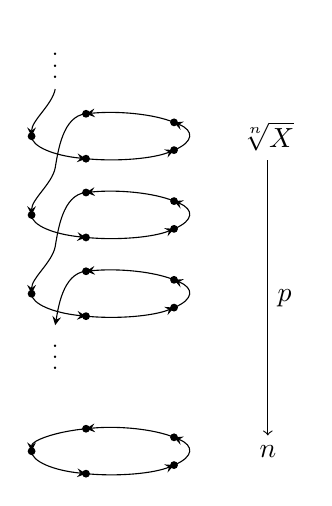
\begin{tikzpicture}
    \node (A) at (2,2) {$\sqrt[n]X$};
    \node (B) at (2,-2) {$\bn{n}$};
    \draw[->] (A) -- node[auto] {$p$} (B);
    \foreach \y in {-2,0,1,2}
    { \begin{scope}[shift={(0,\y)}]
        \foreach \x in {0,...,4}
        { \node[fill,circle,inner sep=1pt] at (180+72*\x:1 and .3) {}; }
        \foreach \x in {0,...,3}
        { \draw[-stealth] (180+72*\x:1 and .3) arc(180+72*\x:252+72*\x:1 and .3); }
      \end{scope} }
    \begin{scope}[shift={(0,-2)}]
      \draw[-stealth] (108:1 and .3) arc(108:180:1 and .3);
    \end{scope}
    \foreach \y in {1,2}
    { \begin{scope}[shift={(0,\y)}]
        \draw[-stealth] (108:1 and .3)
        .. controls ++( 5:-.3) and ++(80:.2) .. (-.7,-.4)
        .. controls ++(80:-.2) and ++(90:.2) .. (-1,-1);
      \end{scope} }
    \draw[-stealth] (108:1 and .3)
    .. controls ++( 5:-.3) and ++(80:.2) .. (-.7,-.4);
    \node (dz) at (-.7,-.7) {\footnotesize $\vdots$};
    \begin{scope}[shift={(0,3)}]
      \draw[-stealth] (-.7,-.4)
      .. controls ++(80:-.2) and ++(90:.2) .. (-1,-1);
    \node (da) at (-.7,0) {\footnotesize $\vdots$};
    \end{scope}
  \end{tikzpicture}
  \caption{The $n$'th root of an endomorphism, with projection}
  \label{fig:rootproj}
\end{figure}
